\documentclass[11pt,letterpaper]{article}
\usepackage[margin=0.8in,top=0.85in,bottom=0.8in]{geometry}
\usepackage[T1]{fontenc}
\usepackage[utf8]{inputenc}
\usepackage{newtxtext,newtxmath,microtype,graphicx,booktabs,longtable,array,tabularx,multirow,xcolor,fancyhdr,lastpage,pdflscape,caption,tocloft,hyperref,colortbl}
\hypersetup{colorlinks=true,linkcolor=black,urlcolor=blue,pdftitle=Reserve Management Plan}
\definecolor{linegray}{HTML}{C8CDD2}
\definecolor{sectionblue}{HTML}{3A5F7D}
\definecolor{softgray}{HTML}{F6F7F8}
\setlength{\headheight}{16pt}
\pagestyle{fancy}
\fancyhf{}
\fancyhead[L]{\footnotesize Ridge Park Luxury Condominiums Owners' Association Inc.}
\fancyhead[R]{\footnotesize January 1, 2025}
\fancyfoot[L]{\footnotesize Reserve Study Report}
\fancyfoot[R]{\footnotesize Page \thepage\ of \pageref{LastPage}}
\setlength{\parindent}{0pt}
\setlength{\parskip}{0.45em}
\renewcommand{\arraystretch}{1.18}

\newcommand{\sectionrule}{\par\vspace{0.2em}{\color{linegray}\rule{\linewidth}{0.6pt}}\par\vspace{0.6em}}
\newcommand{\reportsection}[1]{%
  \par\vspace{0.2em}%
  \addcontentsline{toc}{section}{#1}%
  {{\Large\bfseries\color{sectionblue} #1\par}}%
  \sectionrule
}
\newcommand{\subnote}[1]{\vspace{0.3em}\colorbox{softgray}{\parbox{0.97\linewidth}{\small #1}}\vspace{0.4em}}

\begin{document}

\thispagestyle{empty}
\begin{flushleft}
{\small Board of Directors}\\
{\small Ridge Park Luxury Condominiums Owners' Association Inc.}\\
{\small Los Alamos, New Mexico}
\end{flushleft}

\vspace{0.8em}
Please find attached your reserve study report. This version was generated from association CSV source files using a Python-to-LaTeX workflow so that the report can be reproduced, updated, and audited from the underlying data package.

The report is intended to mirror the structure and feel of a conventional reserve study: a cover page, statement of position, component summaries, annual funding projections, expenditure schedules, and supporting disclosures. The purpose is not to imitate the original preparer’s authorship, but to provide a transparent and reusable reporting format driven directly by the uploaded reserve data.

The reserve model remains a planning tool rather than a prediction of exact future outcomes. Actual repair timing, pricing, inflation, and investment returns will differ from the assumptions used here. The goal is to keep the association approximately funded at approximately the right time and to make long-range reserve decisions easier to review.

Sincerely,\\[0.7em]
Brendan J. Gifford\\
Ridge Park Treasurer
\newpage

\thispagestyle{empty}
\begin{center}
\vspace*{1.2cm}
{\LARGE\bfseries Ridge Park Luxury Condominiums Owners' Association Inc.}\\[2.0cm]
{\Huge\bfseries Reserve Management Plan}\\[0.45cm]
{\Large\bfseries Type 1}\\[0.45cm]
{\LARGE\bfseries Reserve Study with Data-Driven Analysis}\\[1.7cm]
{\large\bfseries For 30-Year Projection Period Beginning January 1, 2025}\\[1.0cm]
\IfFileExists{cover_img.png}{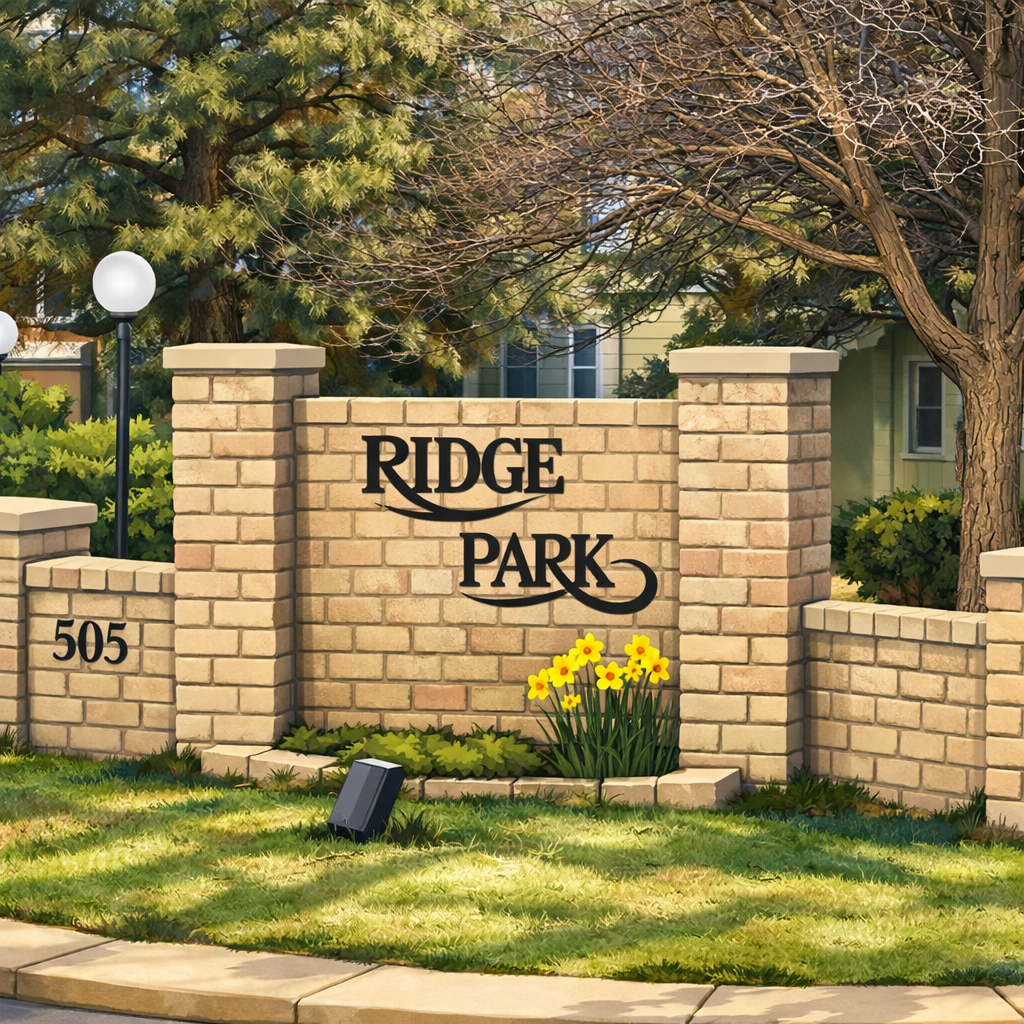
\includegraphics[width=0.68\linewidth]{cover_img.png}}{\vspace{3cm}}
\end{center}
\newpage

\tableofcontents
\newpage

\reportsection{Preparer's Report on Reserve Study}
{\bfseries Description of Engagement and Report}\\
This report was generated from the uploaded CSV data package for the association. The workflow reads the reserve assumptions, component inventory, replacement schedule, annual contribution plan, and reserve cash-flow projection, then renders a formatted LaTeX report designed to resemble a traditional reserve study binder. It is intended as a reproducible reporting layer over the association's source data.

{\bfseries Management's Responsibility}\\
Management remains responsible for the assumptions underlying the reserve model, including inflation, investment return, beginning reserve balance, component scope, useful life estimates, replacement timing, and any planned contribution or special assessment strategy.

{\bfseries Generator Responsibility}\\
The generator's responsibility is limited to organizing the supplied data into financial exhibits, narrative disclosures, and summary schedules. It does not perform a site inspection, engineering opinion, destructive testing, or warranty analysis.

{\bfseries Important Limitations}\\
This report should be read together with the source CSV package. If the underlying source data changes, the PDF should be regenerated so that tables and summary metrics remain aligned with the current model.

\subnote{This version is not prepared by a credentialed professional. It is best treated as a transparent analytical report, not as a substitute for engineering judgment or legal advice.}

\newpage
\reportsection{Statement of Position}
\begin{tabularx}{\linewidth}{>{\bfseries}l X}
Projection period: & 2025 to 2054 \\
Type of project: & Reserve Study \\
Number of units: & 138 \\
Location: & Los Alamos, New Mexico \\
Project construction date: & 1984 \\
Analysis date: & January 1, 2025 \\
Report prepared by: & Brendan J. Gifford, Treasurer \\
\end{tabularx}

\vspace{0.8em}
\begin{tabularx}{\linewidth}{X r}
\toprule
Metric & Value \\
\midrule
\rowcolor{blue!12} Current Replacement Cost & \$6,246,134 \\
Future Replacement Cost & \$7,435,954 \\
\rowcolor{blue!12} Current Reserve Fund Balance & \$220,000 \\
Fully Funded Reserve Balance & \$4,647,235 \\
\rowcolor{blue!12} Percent Funded & 4.73 \% \\
Reserve Deficit & \$4,427,235 \\
\rowcolor{blue!12} Reserve Deficit per Unit & \$32,081 \\
Projected Annual Reserve Contribution & \$805,200 \\
\rowcolor{blue!12} Average Annual Reserve Contribution per Unit & \$435 \\
Projected Monthly Reserve Contribution & \$5,000 \\
\rowcolor{blue!12} Average Monthly Reserve Contribution per Unit & \$36 \\
\bottomrule
\end{tabularx}

\subnote{First-year reserve contribution: \$60,000. First-year ending balance: \$339,784. Ending balance in the final projection year (2054): \$5,720,900.}

\newpage
\reportsection{Summary of Major Components}
{\small Analysis Date - January 1, 2025 \quad Inflation: 3.00\% \quad Investment: 2.00\% \quad Contribution Factor: 0.00}

\vspace{0.6em}
\begin{tabularx}{\linewidth}{X >{\centering\arraybackslash}p{1.3cm} >{\centering\arraybackslash}p{2.2cm} >{\centering\arraybackslash}p{2.3cm} >{\raggedleft\arraybackslash}p{2.7cm}}
\toprule
Category & Useful Lives & Replacement Years & Remaining Years & Future Cost \\
\midrule
\rowcolor{blue!12} Exterior Surfaces & 7-30 & 2025-2039 & 0:06-14:06 & \$2,540,353 \\
Roofing & 5-30 & 2025-2035 & 0:06-10:06 & \$1,783,581 \\
\rowcolor{blue!12} Asphalt & 3-30 & 2025-2045 & 0:06-20:06 & \$1,242,739 \\
Painting & 7-12 & 2025-2031 & 0:06-6:06 & \$822,831 \\
\rowcolor{blue!12} Balconies-Decks-Stairways & 5-20 & 2025-2030 & 0:06-5:06 & \$431,941 \\
Doors-Windows & 7-25 & 2027-2035 & 2:06-10:06 & \$196,995 \\
\rowcolor{blue!12} Flooring & 12-20 & 2030-2034 & 5:06-9:06 & \$74,026 \\
Fire Safety & 3-5 & 2025-2028 & 0:06-3:06 & \$63,597 \\
\rowcolor{blue!12} Renovation & 10-20 & 2028-2038 & 3:06-13:06 & \$61,295 \\
Concrete & 3-25 & 2025-2043 & 0:06-18:06 & \$48,231 \\
\rowcolor{blue!12} Equipment & 7-25 & 2027-2035 & 2:06-10:06 & \$37,846 \\
Fences-Walls-Gates & 3-25 & 2025-2035 & 0:06-10:06 & \$35,466 \\
\rowcolor{blue!12} Lighting & 4-20 & 2025-2030 & 0:06-5:06 & \$22,852 \\
Landscape & 1-8 & 2025-2030 & 0:06-5:06 & \$17,150 \\
\rowcolor{blue!12} Interior Furniture & 5-20 & 2027-2030 & 2:06-5:06 & \$13,881 \\
Structural & 5-10 & 2025-2027 & 0:06-2:06 & \$12,995 \\
\rowcolor{blue!12} Appliances & 10-15 & 2027-2030 & 2:06-5:06 & \$9,038 \\
Plumbing & 5-12 & 2026-2034 & 1:06-9:06 & \$8,405 \\
\rowcolor{blue!12} Signage & 5-15 & 2025-2030 & 0:06-5:06 & \$5,492 \\
HVAC & 15-20 & 2030 & 5:06 & \$5,412 \\
\rowcolor{blue!12} Exterior Furniture & 4 & 2026 & 1:06 & \$1,829 \\
\bottomrule
\end{tabularx}

\newpage
\reportsection{Percent Funded - Annual - Ending Balance}
\begin{longtable}{>{\centering\arraybackslash}p{1.4cm} >{\raggedleft\arraybackslash}p{2.6cm} >{\raggedleft\arraybackslash}p{2.7cm} >{\raggedleft\arraybackslash}p{2.0cm}}
\toprule
Year & Ending Balance & Funded Balance & Percent Funded \\
\midrule
\endfirsthead
\toprule
Year & Ending Balance & Funded Balance & Percent Funded \\
\midrule
\endhead
\rowcolor{blue!12} 2025 & \$339,784 & \$4,443,227 & 7.65\% \\
2026 & \$459,010 & \$4,206,299 & 10.91\% \\
\rowcolor{blue!12} 2027 & \$552,186 & \$3,917,523 & 14.10\% \\
2028 & \$685,423 & \$3,636,762 & 18.85\% \\
\rowcolor{blue!12} 2029 & \$872,277 & \$3,370,003 & 25.88\% \\
2030 & \$350,757 & \$3,107,058 & 11.29\% \\
\rowcolor{blue!12} 2031 & \$34,515 & \$3,009,599 & 1.15\% \\
2032 & \$-39,815 & \$3,101,683 & -1.28\% \\
\rowcolor{blue!12} 2033 & \$75,781 & \$3,314,666 & 2.29\% \\
2034 & \$89,884 & \$3,333,562 & 2.70\% \\
\rowcolor{blue!12} 2035 & \$267,660 & \$2,875,415 & 9.31\% \\
2036 & \$550,737 & \$3,025,377 & 18.20\% \\
\rowcolor{blue!12} 2037 & \$698,101 & \$3,051,491 & 22.88\% \\
2038 & \$791,012 & \$3,035,003 & 26.06\% \\
\rowcolor{blue!12} 2039 & \$1,069,557 & \$3,217,814 & 33.24\% \\
2040 & \$1,432,272 & \$3,500,459 & 40.92\% \\
\rowcolor{blue!12} 2041 & \$1,662,800 & \$3,666,922 & 45.35\% \\
2042 & \$2,255,820 & \$4,214,757 & 53.52\% \\
\rowcolor{blue!12} 2043 & \$2,739,127 & \$4,672,598 & 58.62\% \\
2044 & \$3,330,511 & \$5,259,633 & 63.32\% \\
\rowcolor{blue!12} 2045 & \$3,479,880 & \$5,422,842 & 64.17\% \\
2046 & \$3,561,467 & \$5,535,543 & 64.34\% \\
\rowcolor{blue!12} 2047 & \$3,681,768 & \$5,707,557 & 64.51\% \\
2048 & \$3,867,513 & \$5,967,340 & 64.81\% \\
\rowcolor{blue!12} 2049 & \$3,978,125 & \$6,175,283 & 64.42\% \\
2050 & \$3,802,056 & \$6,119,033 & 62.13\% \\
\rowcolor{blue!12} 2051 & \$4,102,503 & \$6,565,235 & 62.49\% \\
2052 & \$4,443,308 & \$7,080,931 & 62.75\% \\
\rowcolor{blue!12} 2053 & \$4,976,948 & \$7,821,498 & 63.63\% \\
2054 & \$5,720,900 & \$8,808,021 & 64.95\% \\
\bottomrule
\end{longtable}

\newpage
\reportsection{Cash Flow - Annual}
\begin{longtable}{>{\centering\arraybackslash}p{1.1cm} >{\raggedleft\arraybackslash}p{2.0cm} >{\raggedleft\arraybackslash}p{1.9cm} >{\raggedleft\arraybackslash}p{2.1cm} >{\raggedleft\arraybackslash}p{1.9cm} >{\raggedleft\arraybackslash}p{1.7cm} >{\raggedleft\arraybackslash}p{2.0cm}}
\toprule
Year & Begin & Contribution & Special Assess. & Expenditures & Interest & Ending \\
\midrule
\endfirsthead
\toprule
Year & Begin & Contribution & Special Assess. & Expenditures & Interest & Ending \\
\midrule
\endhead
\rowcolor{blue!12} 2025 & \$220,000 & \$60,000 & \$745,200 & \$698,447 & \$13,031 & \$339,784 \\
2026 & \$339,784 & \$90,000 & \$745,200 & \$731,474 & \$15,500 & \$459,010 \\
\rowcolor{blue!12} 2027 & \$459,010 & \$112,500 & \$745,200 & \$782,252 & \$17,727 & \$552,186 \\
2028 & \$552,186 & \$140,625 & \$745,200 & \$772,583 & \$19,995 & \$685,423 \\
\rowcolor{blue!12} 2029 & \$685,423 & \$175,781 & \$745,200 & \$757,323 & \$23,195 & \$872,277 \\
2030 & \$872,277 & \$219,727 & \$0 & \$754,935 & \$13,689 & \$350,757 \\
\rowcolor{blue!12} 2031 & \$350,757 & \$274,658 & \$0 & \$595,990 & \$5,090 & \$34,515 \\
2032 & \$34,515 & \$343,323 & \$0 & \$418,592 & \$939 & \$-39,815 \\
\rowcolor{blue!12} 2033 & \$-39,815 & \$429,153 & \$0 & \$314,800 & \$1,242 & \$75,781 \\
2034 & \$75,781 & \$536,442 & \$0 & \$525,323 & \$2,984 & \$89,884 \\
\rowcolor{blue!12} 2035 & \$89,884 & \$670,552 & \$500,000 & \$1,002,759 & \$9,982 & \$267,660 \\
2036 & \$267,660 & \$670,552 & \$0 & \$396,868 & \$9,393 & \$550,737 \\
\rowcolor{blue!12} 2037 & \$550,737 & \$670,552 & \$0 & \$537,122 & \$13,934 & \$698,101 \\
2038 & \$698,101 & \$670,552 & \$0 & \$594,073 & \$16,432 & \$791,012 \\
\rowcolor{blue!12} 2039 & \$791,012 & \$670,552 & \$0 & \$411,840 & \$19,832 & \$1,069,557 \\
2040 & \$1,069,557 & \$670,552 & \$0 & \$333,942 & \$26,105 & \$1,432,272 \\
\rowcolor{blue!12} 2041 & \$1,432,272 & \$670,552 & \$0 & \$472,294 & \$32,269 & \$1,662,800 \\
2042 & \$1,662,800 & \$670,552 & \$0 & \$117,422 & \$39,890 & \$2,255,820 \\
\rowcolor{blue!12} 2043 & \$2,255,820 & \$670,552 & \$0 & \$238,095 & \$50,850 & \$2,739,127 \\
2044 & \$2,739,127 & \$670,552 & \$0 & \$140,590 & \$61,421 & \$3,330,511 \\
\rowcolor{blue!12} 2045 & \$3,330,511 & \$670,552 & \$0 & \$590,777 & \$69,594 & \$3,479,880 \\
2046 & \$3,479,880 & \$670,552 & \$0 & \$660,986 & \$72,021 & \$3,561,467 \\
\rowcolor{blue!12} 2047 & \$3,561,467 & \$670,552 & \$0 & \$624,227 & \$73,976 & \$3,681,768 \\
2048 & \$3,681,768 & \$670,552 & \$0 & \$561,733 & \$76,926 & \$3,867,513 \\
\rowcolor{blue!12} 2049 & \$3,867,513 & \$670,552 & \$0 & \$639,961 & \$80,021 & \$3,978,125 \\
2050 & \$3,978,125 & \$670,552 & \$0 & \$926,479 & \$79,858 & \$3,802,056 \\
\rowcolor{blue!12} 2051 & \$3,802,056 & \$670,552 & \$0 & \$450,391 & \$80,285 & \$4,102,503 \\
2052 & \$4,102,503 & \$670,552 & \$0 & \$416,381 & \$86,634 & \$4,443,308 \\
\rowcolor{blue!12} 2053 & \$4,443,308 & \$670,552 & \$0 & \$231,967 & \$95,055 & \$4,976,948 \\
2054 & \$4,976,948 & \$670,552 & \$0 & \$34,081 & \$107,480 & \$5,720,900 \\
\bottomrule
\end{longtable}

\newpage
\reportsection{Disclosures}
\begin{itemize}
\item This report was generated from CSV source files supplied in the working directory, including assumptions, component inventory, projected expenditures, annual contribution schedules, and reserve cash-flow outputs.
\item Analysis date: January 1, 2025. Projection horizon: 30 years.
\item Inflation assumption used in the model: 3.00\%.
\item Investment return assumption used in the model: 2.00\%.
\item Beginning reserve balance used in the projection: \$220,000.
\item Component replacement timing and cost estimates come from the uploaded component list and replacement schedule. Actual field conditions may cause different timing or scope.
\item This document is formatted to resemble a conventional reserve study, but it is produced from the association's current analytical dataset rather than from proprietary reserve-study software.
\item Readers should review contribution levels, projected expenditures, and percent-funded results together. No single table should be interpreted in isolation.
\end{itemize}

\newpage
\begin{landscape}
\reportsection{Expenditures Matrix: Years 1--10}
\scriptsize
\setlength{\tabcolsep}{4.0pt}
\begin{tabular}{p{4.2cm}*{10}{r}}
\toprule
Category & 2025 & 2026 & 2027 & 2028 & 2029 & 2030 & 2031 & 2032 & 2033 & 2034 \\
\midrule
\rowcolor{blue!12} Appliances &  &  & \$2,584 & \$2,218 &  & \$4,236 &  &  &  &  \\
Asphalt & \$121,787 & \$193,387 & \$129,204 & \$133,080 & \$211,319 &  & \$90,887 & \$81,132 &  &  \\
\rowcolor{blue!12} Balconies-Decks-Stairways & \$58,356 & \$60,107 & \$113,053 & \$67,094 & \$65,680 & \$67,651 &  & \$31,205 &  & \$19,863 \\
Concrete & \$15,223 &  &  & \$16,635 &  &  & \$18,177 &  &  & \$19,863 \\
\rowcolor{blue!12} Doors-Windows &  &  & \$4,845 & \$3,881 & \$2,285 & \$31,766 & \$27,872 & \$34,949 & \$29,570 & \$36,416 \\
Equipment &  &  & \$14,675 & \$499 & \$1,713 & \$3,000 & \$909 &  &  & \$9,932 \\
\rowcolor{blue!12} Exterior Furniture &  & \$1,829 &  &  &  & \$2,059 &  &  &  & \$2,317 \\
Exterior Surfaces & \$58,356 & \$70,560 & \$61,910 & \$63,767 & \$77,103 & \$350,019 & \$181,775 & \$193,469 & \$192,845 & \$211,872 \\
\rowcolor{blue!12} Fences-Walls-Gates & \$5,074 &  & \$1,615 & \$11,090 &  & \$2,941 & \$3,030 & \$1,872 & \$6,428 & \$3,310 \\
Fire Safety & \$58,052 &  &  & \$66,762 &  & \$2,353 & \$66,893 &  & \$6,428 & \$73,096 \\
\rowcolor{blue!12} Flooring &  &  &  &  &  & \$26,354 &  &  &  & \$47,671 \\
HVAC &  &  &  &  &  & \$5,412 &  &  &  &  \\
\rowcolor{blue!12} Interior Furniture &  &  & \$6,999 &  &  & \$6,883 &  & \$1,872 &  &  \\
Landscape & \$14,208 & \$8,363 & \$8,614 & \$15,526 & \$9,138 & \$12,354 & \$16,966 & \$9,985 & \$10,285 & \$18,539 \\
\rowcolor{blue!12} Lighting & \$4,567 &  & \$9,152 & \$5,545 & \$1,713 & \$5,353 &  &  & \$1,928 & \$11,256 \\
Painting & \$104,534 & \$141,120 & \$107,670 & \$116,445 & \$114,227 & \$117,653 & \$121,183 &  &  &  \\
\rowcolor{blue!12} Plumbing &  & \$5,227 &  &  &  &  & \$6,059 &  &  & \$3,178 \\
Renovation &  &  &  & \$2,772 &  & \$37,061 &  &  &  &  \\
\rowcolor{blue!12} Roofing & \$248,648 & \$250,881 & \$316,549 & \$266,159 & \$274,144 & \$66,309 & \$62,240 & \$64,107 & \$66,030 & \$68,011 \\
Signage & \$2,030 &  &  & \$1,109 &  & \$4,706 &  &  & \$1,286 &  \\
\rowcolor{blue!12} Structural & \$7,612 &  & \$5,383 &  &  & \$8,824 &  &  &  &  \\
\bottomrule
\end{tabular}
\end{landscape}

\newpage
\begin{landscape}
\reportsection{Expenditures Matrix: Years 11--20}
\scriptsize
\setlength{\tabcolsep}{4.0pt}
\begin{tabular}{p{4.2cm}*{10}{r}}
\toprule
Category & 2035 & 2036 & 2037 & 2038 & 2039 & 2040 & 2041 & 2042 & 2043 & 2044 \\
\midrule
\rowcolor{blue!12} Appliances &  &  &  & \$2,981 & \$3,684 &  &  &  &  &  \\
Asphalt & \$415,997 &  &  & \$96,876 &  &  & \$228,004 &  &  & \$115,675 \\
\rowcolor{blue!12} Balconies-Decks-Stairways & \$10,229 & \$4,215 & \$36,175 &  &  &  & \$24,429 & \$41,936 & \$12,958 & \$5,339 \\
Concrete &  &  & \$21,705 &  &  & \$23,717 &  &  & \$58,924 &  \\
\rowcolor{blue!12} Doors-Windows & \$31,370 & \$2,810 &  & \$5,216 &  & \$6,325 & \$7,329 & \$8,387 & \$3,456 &  \\
Equipment & \$17,049 & \$2,107 &  & \$671 & \$4,421 &  & \$12,214 & \$5,452 & \$2,592 &  \\
\rowcolor{blue!12} Exterior Furniture &  &  &  & \$2,608 &  &  &  & \$2,936 &  &  \\
Exterior Surfaces & \$210,317 & \$224,775 & \$217,048 & \$223,560 & \$230,267 &  &  & \$25,162 & \$17,278 &  \\
\rowcolor{blue!12} Fences-Walls-Gates & \$23,869 &  & \$5,788 & \$11,178 &  & \$7,906 &  & \$2,516 & \$12,958 &  \\
Fire Safety & \$2,728 &  & \$79,874 & \$7,452 &  & \$90,443 &  &  & \$104,012 &  \\
\rowcolor{blue!12} Flooring &  &  &  &  &  &  &  &  &  &  \\
HVAC &  &  &  &  &  &  &  &  &  &  \\
\rowcolor{blue!12} Interior Furniture &  &  & \$2,170 &  & \$7,676 &  &  & \$2,516 &  &  \\
Landscape & \$10,911 & \$11,239 & \$20,258 & \$15,649 & \$12,281 & \$22,136 & \$13,029 & \$13,420 & \$24,189 & \$14,237 \\
\rowcolor{blue!12} Lighting & \$6,820 & \$4,215 & \$2,170 &  &  & \$2,372 & \$16,286 & \$6,710 &  & \$5,339 \\
Painting & \$147,304 & \$140,484 & \$144,699 & \$201,204 & \$153,511 & \$158,116 & \$162,860 & \$8,387 &  &  \\
\rowcolor{blue!12} Plumbing &  & \$7,024 &  &  &  &  & \$8,143 &  &  &  \\
Renovation &  &  &  & \$25,188 &  &  &  &  &  &  \\
\rowcolor{blue!12} Roofing & \$113,206 &  &  &  &  & \$7,906 &  &  &  &  \\
Signage & \$2,728 &  &  & \$1,490 &  & \$3,162 &  &  & \$1,728 &  \\
\rowcolor{blue!12} Structural & \$10,229 &  & \$7,235 &  &  & \$11,859 &  &  &  &  \\
\bottomrule
\end{tabular}
\end{landscape}

\newpage
\begin{landscape}
\reportsection{Expenditures Matrix: Years 21--30}
\scriptsize
\setlength{\tabcolsep}{4.0pt}
\begin{tabular}{p{4.2cm}*{10}{r}}
\toprule
Category & 2045 & 2046 & 2047 & 2048 & 2049 & 2050 & 2051 & 2052 & 2053 & 2054 \\
\midrule
\rowcolor{blue!12} Appliances & \$6,599 &  &  & \$4,006 &  &  & \$5,253 &  &  &  \\
Asphalt & \$109,980 &  & \$126,401 &  &  & \$138,122 & \$164,153 &  & \$150,930 &  \\
\rowcolor{blue!12} Balconies-Decks-Stairways & \$105,398 & \$108,560 & \$160,432 & \$145,215 & \$118,626 & \$122,185 & \$16,415 & \$63,122 &  &  \\
Concrete &  & \$28,320 &  &  & \$30,946 &  &  & \$33,815 &  &  \\
\rowcolor{blue!12} Doors-Windows &  &  &  & \$16,024 &  & \$12,750 &  & \$11,272 &  &  \\
Equipment & \$4,674 & \$1,416 &  & \$15,924 &  & \$8,500 & \$6,303 &  &  &  \\
\rowcolor{blue!12} Exterior Furniture &  & \$3,304 &  &  &  & \$3,719 &  &  &  & \$4,185 \\
Exterior Surfaces & \$105,398 & \$108,560 & \$111,816 & \$115,171 & \$118,626 & \$164,684 &  & \$11,272 &  &  \\
\rowcolor{blue!12} Fences-Walls-Gates & \$4,583 & \$4,720 & \$2,917 & \$15,022 & \$5,158 & \$5,312 &  & \$9,017 & \$11,610 &  \\
Fire Safety & \$3,666 & \$104,217 &  & \$10,015 & \$113,881 & \$4,250 &  & \$124,441 & \$11,610 &  \\
\rowcolor{blue!12} Flooring &  & \$67,968 &  &  &  & \$47,599 &  &  &  &  \\
HVAC & \$6,599 &  &  &  &  & \$2,125 &  &  &  &  \\
\rowcolor{blue!12} Interior Furniture & \$1,925 &  & \$2,917 &  &  & \$10,200 & \$10,944 & \$3,382 &  &  \\
Landscape & \$14,664 & \$31,152 & \$15,557 & \$16,024 & \$28,883 & \$17,000 & \$17,510 & \$31,561 & \$18,576 & \$25,112 \\
\rowcolor{blue!12} Lighting & \$8,248 &  &  & \$17,025 & \$7,221 & \$5,419 &  & \$6,763 & \$3,483 & \$4,783 \\
Painting & \$188,799 & \$188,799 & \$194,463 & \$200,297 & \$216,621 & \$286,869 & \$218,870 &  &  &  \\
\rowcolor{blue!12} Plumbing &  & \$13,971 &  &  &  &  & \$10,944 &  &  &  \\
Renovation &  &  &  & \$5,007 &  & \$66,936 &  &  & \$33,437 &  \\
\rowcolor{blue!12} Roofing & \$9,165 &  &  &  &  & \$10,625 &  & \$121,736 &  &  \\
Signage & \$7,332 &  &  & \$2,003 &  & \$4,250 &  &  & \$2,322 &  \\
\rowcolor{blue!12} Structural & \$13,748 &  & \$9,723 &  &  & \$15,937 &  &  &  &  \\
\bottomrule
\end{tabular}
\end{landscape}

\newpage
\reportsection{Component List - Summary}
\scriptsize
\begin{longtable}{p{4.2cm} p{1.6cm} r r r c c r}
\toprule
\textbf{Category} & \textbf{Replace} & \textbf{Basis Cost} & \textbf{Quantity} & \textbf{Current Cost} & \textbf{Est Life} & \textbf{Rem Life} & \textbf{Future Cost} \\
\textbf{Component} & \textbf{Date} &  &  &  &  &  &  \\
\midrule
\endfirsthead
\toprule
\textbf{Category} & \textbf{Replace} & \textbf{Basis Cost} & \textbf{Quantity} & \textbf{Current Cost} & \textbf{Est Life} & \textbf{Rem Life} & \textbf{Future Cost} \\
\textbf{Component} & \textbf{Date} &  &  &  &  &  &  \\
\midrule
\endhead
\multicolumn{8}{l}{\textbf{Appliances}} \\
\rowcolor{blue!12} Dryer & 7/27 & \$800 & 3 & \$2,400 & 12 & 2:06 & \$2,584 \\
Clubhouse Bar Appliances & 7/28 & \$2,000 & 1 & \$2,000 & 10 & 3:06 & \$2,218 \\
\rowcolor{blue!12} Clubhouse Staff Refrigerator & 7/30 & \$1,200 & 1 & \$1,200 & 15 & 5:06 & \$1,412 \\
Washer & 7/30 & \$800 & 3 & \$2,400 & 15 & 5:06 & \$2,824 \\
\addlinespace[1pt] \multicolumn{4}{r}{} & \textbf{\$8,000} & & & \textbf{\$9,038} \\
\addlinespace[6pt]
\multicolumn{8}{l}{\textbf{Asphalt}} \\
\rowcolor{blue!12} Asphalt Remove and Replace & 7/25 - 7/29 & \$6 & 100,000 & \$600,000 & 30 & 0:06-4:06 & \$646,582 \\
Asphalt Crack Seal & 7/26 & \$25,000 & 1 & \$25,000 & 3 & 1:06 & \$26,133 \\
\rowcolor{blue!12} Asphalt Seal Coat & 7/26 & \$0 & 100,000 & \$40,000 & 3 & 1:06 & \$41,813 \\
Asphalt Slurry Seal & 7/31 & \$1 & 100,000 & \$75,000 & 10 & 6:06 & \$90,887 \\
\rowcolor{blue!12} Asphalt Mill and Overlay & 7/35 - 7/45 & \$3 & 100,000 & \$300,000 & 25 & 10:06-20:06 & \$437,322 \\
\addlinespace[1pt] \multicolumn{4}{r}{} & \textbf{\$1,040,000} & & & \textbf{\$1,242,739} \\
\addlinespace[6pt]
\multicolumn{8}{l}{\textbf{Balconies-Decks-Stairways}} \\
Balconies-Decks-Posts/Structural Supports & 7/25 - 7/30 & \$2,500 & 138 & \$345,000 & 20 & 0:06-5:06 & \$377,471 \\
\rowcolor{blue!12} Metal Stairway Flashing/Stringers & 7/27 & \$15,000 & 1 & \$15,000 & 7 & 2:06 & \$16,150 \\
Stairway/Balcony Railing & 7/27 & \$7,500 & 1 & \$7,500 & 8 & 2:06 & \$8,075 \\
\rowcolor{blue!12} Wood Balcony Walls & 7/27 & \$25,000 & 1 & \$25,000 & 5 & 2:06 & \$26,917 \\
Walkway Railing & 7/28 & \$3,000 & 1 & \$3,000 & 8 & 3:06 & \$3,327 \\
\addlinespace[1pt] \multicolumn{4}{r}{} & \textbf{\$395,500} & & & \textbf{\$431,941} \\
\addlinespace[6pt]
\multicolumn{8}{l}{\textbf{Concrete}} \\
\rowcolor{blue!12} Concrete Sidewalks-Stairs-Patios/Grinding-Repairs & 7/25 & \$10,000 & 1 & \$10,000 & 3 & 0:06 & \$10,149 \\
Curbs-Gutters & 7/25 & \$5,000 & 1 & \$5,000 & 3 & 0:06 & \$5,074 \\
\rowcolor{blue!12} Pool Area Concrete Deck & 7/43 & \$12 & 1,592 & \$19,104 & 25 & 18:06 & \$33,008 \\
\addlinespace[1pt] \multicolumn{4}{r}{} & \textbf{\$34,104} & & & \textbf{\$48,231} \\
\addlinespace[6pt]
\multicolumn{8}{l}{\textbf{Doors-Windows}} \\
Clubhouse/Fitness Windows & 7/27 & \$4,500 & 1 & \$4,500 & 7 & 2:06 & \$4,845 \\
\rowcolor{blue!12} Clubhouse Glass Doors & 7/28 & \$3,500 & 1 & \$3,500 & 10 & 3:06 & \$3,881 \\
Clubhouse Blinds & 7/29 & \$2,000 & 1 & \$2,000 & 7 & 4:06 & \$2,285 \\
\rowcolor{blue!12} Clubhouse Sliding Glass Doors & 7/30 & \$4,000 & 1 & \$4,000 & 10 & 5:06 & \$4,706 \\
Unit Front and Screen Doors & 7/30 - 7/35 & \$1,000 & 138 & \$138,000 & 25 & 5:06-10:06 & \$175,037 \\
\rowcolor{blue!12} Clubhouse Bathroom/Interior Doors & 7/32 & \$5,000 & 1 & \$5,000 & 10 & 7:06 & \$6,241 \\
\addlinespace[1pt] \multicolumn{4}{r}{} & \textbf{\$157,000} & & & \textbf{\$196,995} \\
\addlinespace[6pt]
\multicolumn{8}{l}{\textbf{Equipment}} \\
Fitness Center Equipment & 7/27 & \$7,500 & 1 & \$7,500 & 7 & 2:06 & \$8,075 \\
\rowcolor{blue!12} Pool Cover & 7/27 & \$4 & 720 & \$2,880 & 12 & 2:06 & \$3,101 \\
Pool Heater Raypak & 7/27 & \$3,000 & 1 & \$3,000 & 15 & 2:06 & \$3,230 \\
\rowcolor{blue!12} Sauna Heater & 7/27 & \$250 & 1 & \$250 & 15 & 2:06 & \$269 \\
Clubhouse 50" TV & 7/28 & \$450 & 1 & \$450 & 10 & 3:06 & \$499 \\
\rowcolor{blue!12} Pool Misc Pipes Valves & 7/29 & \$1,500 & 1 & \$1,500 & 7 & 4:06 & \$1,713 \\
Pool Filter Hayward & 7/30 & \$1,300 & 1 & \$1,300 & 15 & 5:06 & \$1,530 \\
\rowcolor{blue!12} Pool Rails-Ladder & 7/30 & \$250 & 3 & \$750 & 15 & 5:06 & \$882 \\
Pool Room Compressor & 7/30 & \$500 & 1 & \$500 & 15 & 5:06 & \$588 \\
\rowcolor{blue!12} Pool Pump Hayward & 7/31 & \$750 & 1 & \$750 & 15 & 6:06 & \$909 \\
Mail Boxes & 7/35 & \$10,000 & 1 & \$10,000 & 25 & 10:06 & \$13,639 \\
\rowcolor{blue!12} Pool Chemical Controller-Rola Chem & 7/35 & \$2,500 & 1 & \$2,500 & 15 & 10:06 & \$3,410 \\
\addlinespace[1pt] \multicolumn{4}{r}{} & \textbf{\$31,380} & & & \textbf{\$37,846} \\
\addlinespace[6pt]
\multicolumn{8}{l}{\textbf{Exterior Furniture}} \\
Pool Chairs-Tables-Chaise Lounge & 7/26 & \$1,750 & 1 & \$1,750 & 4 & 1:06 & \$1,829 \\
\addlinespace[1pt] \multicolumn{4}{r}{} & \textbf{\$1,750} & & & \textbf{\$1,829} \\
\addlinespace[6pt]
\multicolumn{8}{l}{\textbf{Exterior Surfaces}} \\
\rowcolor{blue!12} Chimney Chases Structural Renovations & 7/25 - 7/30 & \$2,500 & 138 & \$345,000 & 20 & 0:06-5:06 & \$377,471 \\
Fascia-Flashing-Soffits & 7/26 & \$10,000 & 1 & \$10,000 & 8 & 1:06 & \$10,453 \\
\rowcolor{blue!12} Stucco Siding Repair & 7/29 & \$10,000 & 1 & \$10,000 & 7 & 4:06 & \$11,423 \\
Clubhouse Siding & 7/30 & \$12 & 7,500 & \$90,000 & 30 & 5:06 & \$105,888 \\
\rowcolor{blue!12} Wood Siding & 7/30 - 7/39 & \$12 & 125,000 & \$1,500,000 & 30 & 5:06-14:06 & \$2,023,148 \\
Corrugated Balcony Walls & 7/32 & \$5,000 & 1 & \$5,000 & 10 & 7:06 & \$6,241 \\
\rowcolor{blue!12} Pool Coping & 7/35 & \$35 & 120 & \$4,200 & 20 & 10:06 & \$5,728 \\
\addlinespace[1pt] \multicolumn{4}{r}{} & \textbf{\$1,964,200} & & & \textbf{\$2,540,353} \\
\addlinespace[6pt]
\multicolumn{8}{l}{\textbf{Fences-Walls-Gates}} \\
Concrete Brick Grouted Wall & 7/25 & \$2,500 & 1 & \$2,500 & 3 & 0:06 & \$2,537 \\
\rowcolor{blue!12} Pool Area Wall Repair & 7/25 & \$2,500 & 1 & \$2,500 & 5 & 0:06 & \$2,537 \\
Stacked Concrete Block Wall & 7/27 & \$1,500 & 1 & \$1,500 & 5 & 2:06 & \$1,615 \\
\rowcolor{blue!12} Chain Link Fence & 7/28 & \$2,500 & 1 & \$2,500 & 10 & 3:06 & \$2,772 \\
Wooden Perimeter Fence & 7/28 & \$5,000 & 1 & \$5,000 & 5 & 3:06 & \$5,545 \\
\rowcolor{blue!12} Pool Area Metal Rail Fence-Gate & 7/35 & \$75 & 200 & \$15,000 & 25 & 10:06 & \$20,459 \\
\addlinespace[1pt] \multicolumn{4}{r}{} & \textbf{\$29,000} & & & \textbf{\$35,466} \\
\addlinespace[6pt]
\multicolumn{8}{l}{\textbf{Fire Safety}} \\
Chimney Cleaning & 7/25 & \$200 & 138 & \$27,600 & 3 & 0:06 & \$28,011 \\
\rowcolor{blue!12} Dryer Vent Cleaning & 7/25 & \$200 & 138 & \$27,600 & 3 & 0:06 & \$28,011 \\
Fire Extinguishers & 7/25 & \$2,000 & 1 & \$2,000 & 5 & 0:06 & \$2,030 \\
\rowcolor{blue!12} Chimney Flues-Caps-Spark Arrestors & 7/28 & \$5,000 & 1 & \$5,000 & 5 & 3:06 & \$5,545 \\
\addlinespace[1pt] \multicolumn{4}{r}{} & \textbf{\$62,200} & & & \textbf{\$63,597} \\
\addlinespace[6pt]
\multicolumn{8}{l}{\textbf{Flooring}} \\
Clubhouse Tile Floor & 7/30 & \$16 & 1,000 & \$16,000 & 20 & 5:06 & \$18,825 \\
\rowcolor{blue!12} Pool Area Tile Exterior & 7/30 & \$16 & 400 & \$6,400 & 20 & 5:06 & \$7,530 \\
Clubhouse Carpet & 7/34 & \$9 & 4,000 & \$36,000 & 12 & 9:06 & \$47,671 \\
\addlinespace[1pt] \multicolumn{4}{r}{} & \textbf{\$58,400} & & & \textbf{\$74,026} \\
\addlinespace[6pt]
\multicolumn{8}{l}{\textbf{HVAC}} \\
\rowcolor{blue!12} Clubhouse Fireplace & 7/30 & \$1,000 & 1 & \$1,000 & 20 & 5:06 & \$1,177 \\
Clubhouse Furnace & 7/30 & \$1,200 & 3 & \$3,600 & 15 & 5:06 & \$4,236 \\
\addlinespace[1pt] \multicolumn{4}{r}{} & \textbf{\$4,600} & & & \textbf{\$5,412} \\
\addlinespace[6pt]
\multicolumn{8}{l}{\textbf{Interior Furniture}} \\
\rowcolor{blue!12} Clubhouse Folding Tables-Chairs & 7/27 & \$1,500 & 1 & \$1,500 & 5 & 2:06 & \$1,615 \\
Clubhouse Sofa-Chairs & 7/27 & \$5,000 & 1 & \$5,000 & 12 & 2:06 & \$5,383 \\
\rowcolor{blue!12} Clubhouse Barstools & 7/30 & \$350 & 3 & \$1,050 & 15 & 5:06 & \$1,235 \\
Clubhouse Table and Chairs & 7/30 & \$1,600 & 3 & \$4,800 & 20 & 5:06 & \$5,647 \\
\addlinespace[1pt] \multicolumn{4}{r}{} & \textbf{\$12,350} & & & \textbf{\$13,881} \\
\addlinespace[6pt]
\multicolumn{8}{l}{\textbf{Landscape}} \\
\rowcolor{blue!12} Irrigation Control Valves-Sprinkers-Timers & 7/25 & \$2,500 & 1 & \$2,500 & 3 & 0:06 & \$2,537 \\
Landscape Border Blocks & 7/25 & \$1,000 & 1 & \$1,000 & 3 & 0:06 & \$1,015 \\
\rowcolor{blue!12} Landscape Replenishment & 7/25 & \$2,500 & 1 & \$2,500 & 3 & 0:06 & \$2,537 \\
Tree Removal-Major Trimming & 7/25 & \$8,000 & 1 & \$8,000 & 1 & 0:06 & \$8,119 \\
\rowcolor{blue!12} Landscape Rock & 7/30 & \$2,500 & 1 & \$2,500 & 8 & 5:06 & \$2,941 \\
\addlinespace[1pt] \multicolumn{4}{r}{} & \textbf{\$16,500} & & & \textbf{\$17,150} \\
\addlinespace[6pt]
\multicolumn{8}{l}{\textbf{Lighting}} \\
Carport Flood Lights & 7/25 & \$1,500 & 1 & \$1,500 & 4 & 0:06 & \$1,522 \\
\rowcolor{blue!12} Clubhouse Ceiling Fans & 7/25 & \$1,500 & 1 & \$1,500 & 10 & 0:06 & \$1,522 \\
Clubhouse Emergency Lighting & 7/25 & \$1,500 & 1 & \$1,500 & 5 & 0:06 & \$1,522 \\
\rowcolor{blue!12} Clubhouse Interior Lighting & 7/27 & \$3,500 & 1 & \$3,500 & 7 & 2:06 & \$3,768 \\
Pole Globe Lights & 7/27 & \$5,000 & 1 & \$5,000 & 7 & 2:06 & \$5,383 \\
\rowcolor{blue!12} Carport Flourescent Lights & 7/28 & \$2,000 & 1 & \$2,000 & 7 & 3:06 & \$2,218 \\
Lighting Exterior Sconces & 7/28 & \$3,000 & 1 & \$3,000 & 8 & 3:06 & \$3,327 \\
\rowcolor{blue!12} Exterior Globe Wall Lighting & 7/30 & \$2,000 & 1 & \$2,000 & 12 & 5:06 & \$2,353 \\
Pool Area Cage Lights Lights & 7/30 & \$175 & 6 & \$1,050 & 20 & 5:06 & \$1,235 \\
\addlinespace[1pt] \multicolumn{4}{r}{} & \textbf{\$21,050} & & & \textbf{\$22,852} \\
\addlinespace[6pt]
\multicolumn{8}{l}{\textbf{Painting}} \\
\rowcolor{blue!12} Painting Unit Buildings-Clubhouse-Exterior & 7/25 - 7/31 & \$4 & 175,000 & \$700,000 & 10 & 0:06-6:06 & \$777,655 \\
Pool Area Metal Rail Fence-Gate-Painting & 7/25 & \$15 & 200 & \$3,000 & 10 & 0:06 & \$3,045 \\
\rowcolor{blue!12} Clubhouse Interior Painting & 7/26 & \$2 & 20,000 & \$35,000 & 12 & 1:06 & \$36,587 \\
Parking Striping-Curb Painting & 7/28 & \$5,000 & 1 & \$5,000 & 7 & 3:06 & \$5,545 \\
\addlinespace[1pt] \multicolumn{4}{r}{} & \textbf{\$743,000} & & & \textbf{\$822,831} \\
\addlinespace[6pt]
\multicolumn{8}{l}{\textbf{Plumbing}} \\
\rowcolor{blue!12} Sewer Lateral Lines-Cleanouts & 7/26 & \$5,000 & 1 & \$5,000 & 5 & 1:06 & \$5,227 \\
Clubhouse Hot Water Heaters-Expansion & 7/34 & \$1,200 & 2 & \$2,400 & 12 & 9:06 & \$3,178 \\
\addlinespace[1pt] \multicolumn{4}{r}{} & \textbf{\$7,400} & & & \textbf{\$8,405} \\
\addlinespace[6pt]
\multicolumn{8}{l}{\textbf{Renovation}} \\
\rowcolor{blue!12} Clubhouse Maintenance Shop Remodel & 7/28 & \$2,500 & 1 & \$2,500 & 10 & 3:06 & \$2,772 \\
Clubhouse Bar Remodel & 7/30 & \$5,000 & 1 & \$5,000 & 20 & 5:06 & \$5,883 \\
\rowcolor{blue!12} Clubhouse Bathroom Remodel & 7/30 & \$6,000 & 2 & \$12,000 & 20 & 5:06 & \$14,118 \\
Clubhouse Pool Room-Shower Remodel & 7/30 & \$5,000 & 1 & \$5,000 & 20 & 5:06 & \$5,883 \\
\rowcolor{blue!12} Fitness Room Kitchenette Remodel & 7/30 & \$3,500 & 1 & \$3,500 & 20 & 5:06 & \$4,118 \\
Laundry Room Remodel & 7/30 & \$3,500 & 1 & \$3,500 & 20 & 5:06 & \$4,118 \\
\rowcolor{blue!12} Sauna Remodel & 7/30 & \$2,500 & 1 & \$2,500 & 20 & 5:06 & \$2,941 \\
Pool Resurface & 7/38 & \$12 & 1,200 & \$14,400 & 15 & 13:06 & \$21,462 \\
\addlinespace[1pt] \multicolumn{4}{r}{} & \textbf{\$48,400} & & & \textbf{\$61,295} \\
\addlinespace[6pt]
\multicolumn{8}{l}{\textbf{Roofing}} \\
\rowcolor{blue!12} Gutters-Downspouts & 7/25 & \$5,000 & 1 & \$5,000 & 5 & 0:06 & \$5,074 \\
Unit Building Shingle Roofs & 7/25 - 7/29 & \$12 & 100,000 & \$1,200,000 & 30 & 0:06-4:06 & \$1,293,164 \\
\rowcolor{blue!12} Clubhouse Roof & 7/27 & \$12 & 4,500 & \$54,000 & 25 & 2:06 & \$58,142 \\
Carport Roofs & 7/30 - 7/34 & \$12 & 21,400 & \$256,800 & 25 & 5:06-9:06 & \$320,814 \\
\rowcolor{blue!12} Garage Flat Roof & 7/35 & \$6,000 & 13 & \$78,000 & 25 & 10:06 & \$106,386 \\
\addlinespace[1pt] \multicolumn{4}{r}{} & \textbf{\$1,593,800} & & & \textbf{\$1,783,581} \\
\addlinespace[6pt]
\multicolumn{8}{l}{\textbf{Signage}} \\
Building Signs/Numbers & 7/25 & \$2,000 & 1 & \$2,000 & 5 & 0:06 & \$2,030 \\
\rowcolor{blue!12} Misc and Parking Signs & 7/28 & \$1,000 & 1 & \$1,000 & 5 & 3:06 & \$1,109 \\
Monument Sign/Wall & 7/30 & \$2,000 & 1 & \$2,000 & 15 & 5:06 & \$2,353 \\
\addlinespace[1pt] \multicolumn{4}{r}{} & \textbf{\$5,000} & & & \textbf{\$5,492} \\
\addlinespace[6pt]
\multicolumn{8}{l}{\textbf{Structural}} \\
\rowcolor{blue!12} Trash Enclosures & 7/25 & \$7,500 & 1 & \$7,500 & 5 & 0:06 & \$7,612 \\
Carport Support Posts-Beams & 7/27 & \$5,000 & 1 & \$5,000 & 10 & 2:06 & \$5,383 \\
\addlinespace[1pt] \multicolumn{4}{r}{} & \textbf{\$12,500} & & & \textbf{\$12,995} \\
\addlinespace[6pt]
\bottomrule
\end{longtable}

\newpage
\reportsection{Upcoming Major Components}
\begin{longtable}{>{\centering\arraybackslash}p{2.0cm} p{2.6cm} p{7.0cm} >{\raggedleft\arraybackslash}p{2.3cm}}
\toprule
Date & Category & Component & Future Cost \\
\midrule
\endfirsthead
\toprule
Date & Category & Component & Future Cost \\
\midrule
\endhead
\rowcolor{blue!12} 2025-07-01 & Roofing & Unit Building Shingle Roofs & \$243,573 \\
2025-07-01 & Asphalt & Asphalt Remove and Replace & \$121,787 \\
\rowcolor{blue!12} 2025-07-01 & Painting & Painting Unit Buildings-Clubhouse-Exterior & \$101,489 \\
2025-07-01 & Balconies-Decks-Stairways & Balconies-Decks-Posts/Structural Supports & \$58,356 \\
\rowcolor{blue!12} 2025-07-01 & Exterior Surfaces & Chimney Chases Structural Renovations & \$58,356 \\
2025-07-01 & Fire Safety & Chimney Cleaning & \$28,011 \\
\rowcolor{blue!12} 2025-07-01 & Fire Safety & Dryer Vent Cleaning & \$28,011 \\
2025-07-01 & Concrete & Concrete Sidewalks-Stairs-Patios/Grinding-Repairs & \$10,149 \\
\rowcolor{blue!12} 2025-07-01 & Landscape & Tree Removal-Major Trimming & \$8,119 \\
2025-07-01 & Structural & Trash Enclosures & \$7,612 \\
\rowcolor{blue!12} 2025-07-01 & Concrete & Curbs-Gutters & \$5,074 \\
2025-07-01 & Roofing & Gutters-Downspouts & \$5,074 \\
\rowcolor{blue!12} 2025-07-01 & Painting & Pool Area Metal Rail Fence-Gate-Painting & \$3,045 \\
2025-07-01 & Fences-Walls-Gates & Concrete Brick Grouted Wall & \$2,537 \\
\rowcolor{blue!12} 2025-07-01 & Fences-Walls-Gates & Pool Area Wall Repair & \$2,537 \\
2025-07-01 & Landscape & Irrigation Control Valves-Sprinkers-Timers & \$2,537 \\
\rowcolor{blue!12} 2025-07-01 & Landscape & Landscape Replenishment & \$2,537 \\
2025-07-01 & Fire Safety & Fire Extinguishers & \$2,030 \\
\bottomrule
\end{longtable}

\subnote{Largest summarized category by future cost: Exterior Surfaces at \$2,540,353. Lowest year-end reserve balance in the projection occurs in 2032, at \$-39,815. Highest projected percent funded occurs in 2054, at 64.95\%.}

\end{document}
